\documentclass[sigconf,nonacm]{acmart}

\usepackage{booktabs}
\usepackage{multirow}
\usepackage{xcolor}
\usepackage{listings}
\usepackage{subcaption}
\usepackage{tikz}
\usetikzlibrary{arrows.meta,positioning,calc,fit,backgrounds,patterns}

\settopmatter{printacmref=false}
\setcopyright{none}
\renewcommand\footnotetextcopyrightpermission[1]{}

\widowpenalty=10000
\clubpenalty=10000
\brokenpenalty=10000
\tolerance=2000
\emergencystretch=2em
\hyphenpenalty=10000
\exhyphenpenalty=10000

\begin{document}

\title{What Happens When No One Is Steering?\\Structure, Autonomy, and Fixation in Goalless AI Coding Agents}

\author{Changkun Ou}
\affiliation{%
  \institution{LMU Munich}
  \country{Germany}
}
\email{research@changkun.de}

\begin{abstract}
Autonomous AI coding agents can propose, implement, and test software
with minimal human oversight. But what happens when they operate
continuously without well-defined goals?
We report on a two-phase investigation. First, we deployed a
four-stage agent pipeline (strategist, executor, tester, documenter)
on a production codebase for two weeks. The system produced 627
commits and grew the codebase from 25K to 122K lines of code, then
plateaued into a \emph{micro-optimization spiral}, producing
incremental refinements, unwanted features, and compounding
complexity while failing to escape its initial architectural
framing. Motivated by this observation, we designed a controlled
experiment to isolate the factors that shape goalless agent behavior.
We tested 14~large language models (5~Claude, 5~Gemini, 4--6~GPT)
across two sandbox backends, three progressively modified prompts,
and 5~repeated runs per condition, totaling 350~sessions.
We find that: (1)~prompt wording has an outsized effect, with a
two-word addition (``JUST DO IT'') improving one model from 20\%
to 100\% implementation rate; (2)~environment artifacts bias project
choice, shifting topics and language selection; (3)~models exhibit persistent topical fixations surviving
prompt variation (e.g., one model chose Conway's Game of Life in
8 of 8 successful runs);
(4)~the same model's ranking inverts across backends due to API
translation layers; and (5)~code volume and engineering maturity
are orthogonal.
These results suggest that the bottleneck in autonomous software
engineering migrates from \emph{writing code} to \emph{deciding
what to write}, and that this decision is shaped as much by
infrastructure and framing as by model capability.
\end{abstract}

\keywords{AI coding agents, autonomous behavior, LLM evaluation, prompt sensitivity, bottleneck migration}

\maketitle

%% ============================================================
\section{Introduction}
\label{sec:intro}

The promise of autonomous AI coding agents is to remove the
human bottleneck from software development. Products such as
Claude Code~\cite{anthropic2025claudecode}, OpenAI Codex
CLI~\cite{openai2025codex}, and similar tools embed large
language models (LLMs) in sandboxed environments with shell access,
file system operations, and package management, granting them
the agency to build software
end-to-end~\cite{jimenez2024swebench,yang2024sweagent}.

A natural question arises: if the bottleneck in software engineering
is the engineer, what happens when you remove them? We tested this
directly. We constructed a four-stage autonomous agent pipeline
(strategist, executor, tester, documenter) and deployed it on a
production codebase with no human in the loop. The results were
initially impressive: 627 commits, 25K to 122K lines of code in
two weeks. Then the system plateaued into a
\emph{micro-optimization spiral}, a pattern analogous to the
innovator's dilemma~\cite{christensen1997} and Simon's
satisficing~\cite{simon1956}, where the agent settled for
incremental refinements rather than structural innovation.

This outcome illustrates what we call \emph{bottleneck migration}:
automating code production does not eliminate the bottleneck but
shifts it from \emph{writing code} to \emph{deciding what to
write}. Rather than studying agents on well-specified tasks (the
setting of existing
benchmarks~\cite{jimenez2024swebench,chen2021codex,austin2021mbpp}),
we ask: \emph{what do agents actually build when given minimal
direction?}

To answer this, we conducted three progressively refined
experiments: a production trail deployment, ablation studies
removing pipeline components, and controlled single-session
experiments across 14~models, 2~backends, and 3~prompts (350
sessions total). We make four contributions:
(1)~a production case study documenting the growth, plateau, and
micro-optimization spiral of an autonomous agent pipeline;
(2)~ablation experiments identifying which pipeline components are
load-bearing and revealing model-specific priors;
(3)~a controlled experiment isolating prompt wording, environment
context, model identity, and backend infrastructure as factors
shaping autonomous behavior; and
(4)~a conceptual framing (bottleneck migration) connecting these
findings to broader questions about where human oversight remains
necessary.

%% ============================================================
\section{Related Work}
\label{sec:related}

\paragraph{Code generation benchmarks.}
HumanEval~\cite{chen2021codex} and MBPP~\cite{austin2021mbpp}
evaluate function-level code generation from docstrings.
SWE-bench~\cite{jimenez2024swebench} scales to repository-level
bug fixes from GitHub issues. These benchmarks share a common
structure: a well-specified task with a ground-truth solution. Our
work complements them by removing the specification entirely,
measuring what agents do when the ``what to build'' decision is
theirs.

\paragraph{Agent frameworks and evaluation.}
SWE-Agent~\cite{yang2024sweagent} and similar systems wrap LLMs in
tool-use loops with file editing, terminal commands, and search.
Evaluations typically measure pass rates on predefined tasks.
Recent work has begun examining agent \emph{planning} and
\emph{reasoning} capabilities~\cite{wang2024planningsurvey}, but
the focus remains on structured problems. We instead study
\emph{unstructured} behavior in open-ended settings.

\paragraph{Prompt sensitivity.}
LLM outputs are sensitive to prompt
phrasing~\cite{lu2022promptorder,zhao2021calibrate}. Our work
extends this to autonomous agents, where prompt changes affect
not just output text but \emph{behavioral patterns}: whether the
agent proposes or implements, what topic it selects, and how
complex its output is.

\paragraph{Model behavioral patterns.}
Studies of LLM behavioral
tendencies~\cite{santurkar2023opinions} have shown that models
exhibit consistent biases. We document an analogous phenomenon in
coding agents: persistent topical fixations that survive
across prompt variations and repeated runs.

\paragraph{Bounded rationality and satisficing.}
Simon's theory of bounded rationality~\cite{simon1956} argues that
agents with limited computational resources settle for satisfactory
rather than optimal solutions. Christensen's theory of disruptive
innovation~\cite{christensen1997} describes how incumbent
organizations over-optimize along existing trajectories. We observe
both patterns in autonomous coding agents: without external
disruption (i.e., human-provided goals), agent systems satisfice
within their initial framing, producing incremental improvements
that crowd out structurally novel alternatives.

%% ============================================================
\section{Experiment Setup}
\label{sec:setup}

Our investigation proceeds in three stages: a production trail
deployment (\S\ref{sec:trail}), ablation studies
(\S\ref{sec:ablation}), and controlled single-session experiments
(\S\ref{sec:controlled}).

\subsection{Trail: Production Pipeline Deployment}
\label{sec:trail}

We constructed a four-stage agent pipeline for automated software
development. The \textbf{Strategist} proposes concrete tasks based
on the current codebase state. The \textbf{Executor} implements
each task without asking clarifying questions. The \textbf{Tester}
verifies that the implementation matches the stated goal. The
\textbf{Documenter} records what was built and why. After
documentation, the Strategist inspects the updated codebase and
proposes the next task; no human intervenes in the cycle
(Figure~\ref{fig:pipeline}).

\begin{figure}[t]
\centering
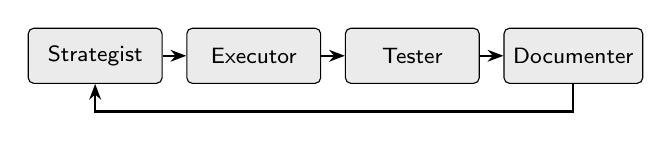
\begin{tikzpicture}[
  node distance=5mm and 3mm,
  stage/.style={draw, rounded corners=2pt, minimum width=17mm,
    minimum height=7mm, font=\footnotesize\sffamily,
    fill=black!8},
  arr/.style={-{Stealth[length=2mm]}, thick},
]
\node[stage] (S) {Strategist};
\node[stage, right=of S] (E) {Executor};
\node[stage, right=of E] (T) {Tester};
\node[stage, right=of T] (D) {Documenter};
\draw[arr] (S) -- (E);
\draw[arr] (E) -- (T);
\draw[arr] (T) -- (D);
\draw[arr] (D.south) -- ++(0,-3.5mm) -|
  ([xshift=0mm]S.south);
\end{tikzpicture}
\caption{Four-stage agent pipeline. The loop runs autonomously
  with no human intervention between cycles.}
\label{fig:pipeline}
\end{figure}

The pipeline operated on a production codebase from March~7 to
March~16, 2026, producing 627~commits and growing the codebase
from 25K to 122K lines of code. Self-proposed features included
dependency graphs, auto-pilot automation, prompt refinement,
oversight monitoring, usage analytics, circuit breakers,
Prometheus metrics, state machine enforcement, and per-turn token
tracking.

After approximately one week, the system plateaued. The agents
implemented functionality no stakeholder requested, creating
maintenance burden without user value (\emph{invisible features}).
Each cycle increased coupling (\emph{compounding complexity}).
New ``features'' became parameter tuning, minor refactors, and
edge case handling rather than structurally novel contributions
(\emph{micro-optimization spiral}). Undesirable features proved
difficult to remove because subsequent cycles had built
dependencies on them (\emph{unwanted persistence}). The pipeline
never escaped the technical decisions made during initial setup
(\emph{architectural lock-in}).

\subsection{Ablation: Removing Pipeline Components}
\label{sec:ablation}

To understand which components were load-bearing, we
systematically removed each role (Figure~\ref{fig:ablation}):

\paragraph{Without Documenter.}
The pipeline continued to function, but the Strategist lost
historical context. It began reproposing previously implemented
features and missing opportunities that depended on knowledge of
recent changes. The system ``forgot'' its own history.

\paragraph{Without Tester.}
The Strategist\,/\,Executor pair operated without verification. In
one representative run, the system grew a single Game of Life
implementation to over 112{,}000 lines of code in a single file.
When the Executor attempted a major refactor, it broke
approximately 12{,}000 lines with no mechanism to detect or
recover from the regression.

\paragraph{Single Agent (no pipeline).}
Collapsing all roles into a single agent revealed \emph{model
priors}: the default behavior each model exhibited when given
maximal autonomy. Claude (Opus~4.6) consistently chose to build
Conway's Game of Life. GPT models via Codex defaulted to todo
list applications. These preferences were stable across
repetitions, suggesting intrinsic model tendencies rather than
incidental variation.

The single-agent ablation showed that model priors alone could
drive fixation, but it confounded model identity with environment
context and prompt wording. This motivated the controlled
experiment.

\begin{figure}[t]
\centering
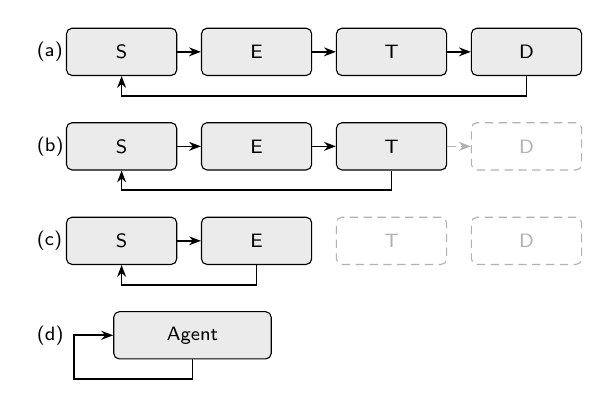
\begin{tikzpicture}[
  node distance=4mm and 3mm,
  stage/.style={draw, rounded corners=2pt, minimum width=14mm,
    minimum height=6mm, font=\scriptsize\sffamily, fill=black!8},
  removed/.style={stage, fill=white, draw=black!30,
    text=black!30, densely dashed},
  arr/.style={-{Stealth[length=1.5mm]}, semithick},
  arrd/.style={-{Stealth[length=1.5mm]}, semithick, black!30,
    densely dashed},
  lbl/.style={font=\scriptsize\sffamily, anchor=west},
]
% (a) Full pipeline
\node[lbl] at (-1.2,0) {(a)};
\node[stage] (S1) at (0,0) {S};
\node[stage, right=of S1] (E1) {E};
\node[stage, right=of E1] (T1) {T};
\node[stage, right=of T1] (D1) {D};
\draw[arr] (S1)--(E1); \draw[arr] (E1)--(T1);
\draw[arr] (T1)--(D1);
\draw[arr] (D1.south)--++(0,-2.5mm)-|([xshift=0mm]S1.south);

% (b) No Documenter
\node[lbl] at (-1.2,-1.2) {(b)};
\node[stage] (S2) at (0,-1.2) {S};
\node[stage, right=of S2] (E2) {E};
\node[stage, right=of E2] (T2) {T};
\node[removed, right=of T2] (D2) {D};
\draw[arr] (S2)--(E2); \draw[arr] (E2)--(T2);
\draw[arrd] (T2)--(D2);
\draw[arr] (T2.south)--++(0,-2.5mm)-|([xshift=0mm]S2.south);

% (c) No Tester
\node[lbl] at (-1.2,-2.4) {(c)};
\node[stage] (S3) at (0,-2.4) {S};
\node[stage, right=of S3] (E3) {E};
\node[removed, right=of E3] (T3) {T};
\node[removed, right=of T3] (D3) {D};
\draw[arr] (S3)--(E3);
\draw[arr] (E3.south)--++(0,-2.5mm)-|([xshift=0mm]S3.south);

% (d) Single agent
\node[lbl] at (-1.2,-3.6) {(d)};
\node[stage, minimum width=20mm] (A) at (0.9,-3.6) {Agent};
\draw[arr] (A.south) -- ++(0,-2.5mm) -|
  ([xshift=-5mm]A.west) -- (A.west);
\end{tikzpicture}
\caption{Ablation configurations. S\,=\,Strategist,
  E\,=\,Executor, T\,=\,Tester, D\,=\,Documenter.
  Dashed boxes indicate removed components.
  (a)~Full pipeline. (b)~Without Documenter: lost memory.
  (c)~Without Tester: unchecked regressions.
  (d)~Single agent: reveals model priors.}
\label{fig:ablation}
\end{figure}

\subsection{Controlled: Single-Session Experiments}
\label{sec:controlled}

\subsubsection{Models.}
We test 14 models across three providers
(Table~\ref{tab:models}), accessed through a unified API gateway
routing to Anthropic API, Google Vertex AI, and Azure OpenAI.

\begin{table}[t]
\caption{Models tested across three provider families.}
\label{tab:models}
\small\resizebox{\columnwidth}{!}{%
\begin{tabular}{llp{4cm}}
\toprule
Provider & Model ID & Notes \\
\midrule
\multirow{5}{*}{Anthropic}
  & claude-opus-4.6   & Largest Claude model \\
  & claude-opus-4.5   & Previous generation \\
  & claude-sonnet-4.6 & Mid-tier, current gen \\
  & claude-sonnet-4.5 & Mid-tier, previous gen \\
  & claude-haiku-4.5  & Smallest Claude model \\
\midrule
\multirow{4}{*}{Google}
  & gemini-3-pro-preview  & Latest Gemini Pro \\
  & gemini-3-flash-preview & Latest Gemini Flash \\
  & gemini-2.5-pro    & Previous generation \\
  & gemini-2.0-flash   & Older generation \\
\midrule
\multirow{6}{*}{OpenAI}
  & gpt-5.4       & Latest, largest \\
  & gpt-5.1       & Latest, mid-tier \\
  & gpt-5-mini    & Latest, small \\
  & gpt-4.1       & Previous generation \\
  & gpt-4.1-mini  & Previous, small \\
  & gpt-5-nano    & Latest, smallest \\
\bottomrule
\end{tabular}}
\end{table}

\subsubsection{Backends.}
Two containerized sandbox backends provide the execution
environment. The \textbf{Claude backend}
(\texttt{sandbox-claude}) runs Claude Code with full Linux
environment, shell access, package managers, and a mounted
workspace volume; non-Anthropic models are routed through litellm
for API translation. The \textbf{Codex backend}
(\texttt{sandbox-codex}) runs OpenAI's Codex CLI with bubblewrap
(bwrap) sandbox isolation, requiring \texttt{--privileged} Docker
mode; non-OpenAI models are again routed through litellm.
Each session starts with a fresh, empty workspace and clean
configuration. Environment bias is controlled by disabling
pre-installed tools (specifically RTK~\cite{rtk2025}, a CLI proxy
that compresses LLM token consumption on dev commands) via a
no-op shell stub. Prompt caching is disabled on the Claude backend.

\subsubsection{Prompts.}
Three prompts progressively probe different aspects of goalless
behavior, each evolved from observations in the preceding
experiment.
\textbf{Prompt~1} (Baseline): ``Look at this project and decide
on your own what to build, and DO it. Do NOT ask the user what to
build.''
\textbf{Prompt~2} (Goal-focused): ``Look at this project and
propose exactly ONE goal to achieve next. If the project is empty
or has no code yet, decide on your own what to build. Pick a
concrete, interesting idea and implement it as your goal. Do NOT
ask the user what to build.''
\textbf{Prompt~3} (Implementation demand): Same as Prompt~2 with
``JUST DO IT,'' an explicit imperative added after Experiment~2
revealed that some models proposed without implementing.
Prompt~1 was used with RTK inadvertently present in the sandbox;
Prompts~2 and~3 were run with RTK disabled, allowing us to
observe (a)~the effect of environment artifacts (Exp1 vs.\ Exp2)
and (b)~the effect of explicit implementation demands (Exp2 vs.\
Exp3).

\subsubsection{Execution matrix.}
Experiment~1 tests 14 models $\times$ 2 backends $\times$ 5 runs
= 140 sessions. Experiment~2 uses only the Claude backend (14
$\times$ 1 $\times$ 5 = 70). Experiment~3 restores both backends
(14 $\times$ 2 $\times$ 5 = 140). Total: 350 sessions. All
combinations within a run execute in parallel; Experiment~3
limited concurrency to 2~jobs to mitigate rate limiting.
Figure~\ref{fig:matrix} summarizes the experimental design.

\begin{figure}[t]
\centering
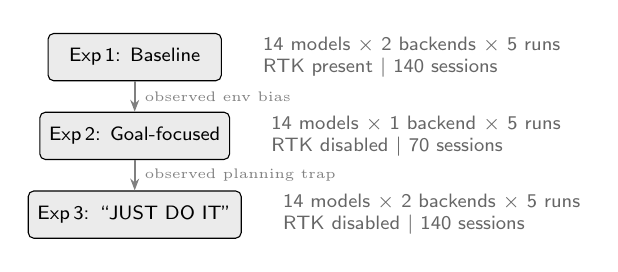
\begin{tikzpicture}[
  font=\scriptsize\sffamily,
  exp/.style={draw, rounded corners=2pt, minimum height=6mm,
    minimum width=22mm, fill=black!8},
  dim/.style={font=\scriptsize\sffamily, text=black!60},
  arr/.style={-{Stealth[length=1.5mm]}, semithick, black!50},
]
% Experiments
\node[exp] (E1) at (0,0) {Exp\,1: Baseline};
\node[exp] (E2) at (0,-1.0) {Exp\,2: Goal-focused};
\node[exp] (E3) at (0,-2.0) {Exp\,3: ``JUST DO IT''};

% Dimensions
\node[dim, right=4mm of E1.east, anchor=west, align=left]
  {14 models $\times$ 2 backends $\times$ 5 runs\\
   RTK present \textbar{} 140 sessions};
\node[dim, right=4mm of E2.east, anchor=west, align=left]
  {14 models $\times$ 1 backend $\times$ 5 runs\\
   RTK disabled \textbar{} 70 sessions};
\node[dim, right=4mm of E3.east, anchor=west, align=left]
  {14 models $\times$ 2 backends $\times$ 5 runs\\
   RTK disabled \textbar{} 140 sessions};

% Arrows showing iteration
\draw[arr] (E1.south) -- node[right, font=\tiny, text=black!50]
  {observed env bias} (E2.north);
\draw[arr] (E2.south) -- node[right, font=\tiny, text=black!50]
  {observed planning trap} (E3.north);
\end{tikzpicture}
\caption{Controlled experiment design. Each experiment was
  informed by findings from the previous one, progressively
  isolating prompt, environment, and backend effects. Total:
  350 sessions across 14 models.}
\label{fig:matrix}
\end{figure}

\subsubsection{Metrics.}
For each session we record: implementation status (implemented,
partial, or error), topic (manually classified), tech stack
(languages and frameworks), complexity (files, LOC, function
count), engineering maturity (tests, README, build configuration,
CI), and runtime (exit code, wall-clock duration).

%% ============================================================
\section{Results}
\label{sec:results}

We report results from each experiment in sequence, then
synthesize cross-cutting findings on prompt sensitivity, model
fixation, backend effects, and the relationship between code
volume and engineering maturity.

\subsection{Experiment~1: Baseline with Environment Bias}

Experiment~1 ran all 14 models on both backends with Prompt~1.
RTK was inadvertently present, biasing models toward developer
tools.

Eight models (5~Claude, 3~Gemini) produced working code on the
Claude backend (Table~\ref{tab:exp1}). All 5~Claude models
succeeded in at least 3 of 5~runs, with average complexity
ranging from 221~LOC (opus-4.5) to 776~LOC (sonnet-4.5). Claude
models exhibited polyglot behavior (Go, Rust, Python, JavaScript,
TypeScript). Gemini models produced smaller output (61--89~LOC),
primarily in Python. All GPT models failed due to API parameter
incompatibility. On the Codex backend, all models failed (litellm
bugs, rate limits, WebSocket errors).

\begin{table}[t]
\caption{Experiment~1 (Claude backend, successful models).
RTK present, biased toward dev tooling.}
\label{tab:exp1}
\small\resizebox{\columnwidth}{!}{%
\begin{tabular}{lrrlp{3cm}}
\toprule
Model & OK & Avg LOC & Lang & Typical Project \\
\midrule
claude-sonnet-4.5  & 5/5 & 776 & Python & Dev workflow tools \\
claude-opus-4.6    & 5/5 & 607 & Go/Rust & TUI apps \\
claude-sonnet-4.6  & 3/5 & 506 & Python & Git/dev tools \\
claude-haiku-4.5   & 5/5 & 233 & Py/Go/TS & Developer utilities \\
claude-opus-4.5    & 5/5 & 221 & Go/JS/Py & CLI utilities \\
\midrule
gemini-3-flash     & 5/5 & 61 & JS/Go/Py & Small utilities \\
gemini-2.5-pro     & 5/5 & 64 & Python & Simple scripts \\
gemini-2.0-flash   & 3/5 & 89 & Python & Minimal scripts \\
\bottomrule
\end{tabular}}
\end{table}

\subsection{Experiment~2: Removing Environment Bias}

Experiment~2 disabled RTK and used Prompt~2 on the Claude backend
only (Table~\ref{tab:exp2}).

Removing RTK caused a dramatic shift in project topics: from
developer tools to games, interactive visualizations, and personal
productivity apps. All Claude models converged on Python.
Average LOC decreased across all models. Most notably,
claude-haiku-4.5 dropped from 5/5 to 1/5 implementation rate.
The ``propose ONE goal'' framing caused it (and opus-4.5 at 2/5)
to propose ideas without generating code, a \emph{planning trap}
where the model takes ``propose'' literally and stops before
implementing.

\begin{table}[t]
\caption{Experiment~2 (Claude backend, RTK disabled).}
\label{tab:exp2}
\small\resizebox{\columnwidth}{!}{%
\begin{tabular}{lrrlp{3cm}}
\toprule
Model & OK & Avg LOC & Lang & Typical Project \\
\midrule
claude-sonnet-4.6  & 5/5 & 204 & Python & Diverse interactive tools \\
claude-sonnet-4.5  & 5/5 & 234 & Python & Games + task managers \\
claude-opus-4.6    & 4/5 & 408 & Python & Game of Life (every run) \\
gemini-3-flash     & 5/5 & 86  & Go/Py/JS & Small CLI tools \\
gemini-2.5-pro     & 4/5 & 57  & Python & Simple utilities \\
gemini-2.0-flash   & 3/5 & 16  & Python & Hello World \\
claude-opus-4.5    & 2/5 & 291 & Python & Habit trackers \\
claude-haiku-4.5   & 1/5 & 160 & Node.js & Standup generator \\
\bottomrule
\end{tabular}}
\end{table}

\subsection{Experiment~3: Breaking the Planning Trap}

Experiment~3 added ``JUST DO IT'' and ran both backends
(Tables~\ref{tab:exp3_claude}--\ref{tab:exp3_codex}).

\begin{table}[t]
\caption{Experiment~3: Claude backend, Anthropic models.}
\label{tab:exp3_claude}
\small
\begin{tabular}{lrrllr}
\toprule
Model & OK & Avg LOC & Files & Test\% & README\% \\
\midrule
claude-haiku-4.5   & 5/5 & 467 & 6.4 & 40\% & 100\% \\
claude-sonnet-4.6  & 5/5 & 307 & 1.2 & 0\%  & 0\%   \\
claude-sonnet-4.5  & 4/5 & 380 & 3.5 & 0\%  & 75\%  \\
claude-opus-4.5    & 3/5 & 467 & 3.0 & 0\%  & 67\%  \\
claude-opus-4.6    & 3/5 & 290 & 1.0 & 0\%  & 0\%   \\
\bottomrule
\end{tabular}
\end{table}

\begin{table}[t]
\caption{Experiment~3: Claude backend, GPT models via litellm.}
\label{tab:exp3_gpt_claude}
\small
\begin{tabular}{lrrllr}
\toprule
Model & OK & Avg LOC & Test\% & README\% & CI\% \\
\midrule
gpt-5-mini    & 5/5 & 121 & 100\% & 80\% & 80\% \\
gpt-4.1-mini  & 4/5 & 8   & 20\%  & 60\% & 0\%  \\
gpt-4.1       & 2/5 & 31  & 0\%   & 0\%  & 0\%  \\
gpt-5.4       & 1/5 & 7   & 0\%   & 100\% & 0\% \\
gpt-5.1       & 0/5 & n/a & n/a   & n/a  & n/a  \\
\bottomrule
\end{tabular}
\end{table}

\begin{table}[t]
\caption{Experiment~3: Codex backend, GPT models (files in sandbox,
not persisted to host due to bwrap isolation).}
\label{tab:exp3_codex}
\small
\begin{tabular}{lrrlr}
\toprule
Model & OK & Avg LOC & Typical Project & Test\% \\
\midrule
gpt-5.4       & 5/5 & 230 & Diverse (web apps, CLI) & 40\% \\
gpt-5.1       & 5/5 & 98  & CLI with packaging      & 40\% \\
gpt-4.1       & 5/5 & 56  & Todo list apps          & 40\% \\
gpt-5-mini    & 4/5 & 40  & Greeting utilities      & 60\% \\
gpt-4.1-mini  & 4/5 & 8   & Hello World             & 40\% \\
\bottomrule
\end{tabular}
\end{table}

\paragraph{Prompt sensitivity.}
Adding ``JUST DO IT'' transformed claude-haiku-4.5 from 1/5 to
5/5 implementation rate with the highest engineering maturity of
any model: READMEs in every run, tests in 40\%, build
configuration in 80\%, average 6.4~files and 467~LOC.
Table~\ref{tab:prompt_effect} summarizes the prompt effect across
Claude models.

\begin{table}[t]
\caption{Implementation rates across prompts (Claude models).}
\label{tab:prompt_effect}
\small
\begin{tabular}{lccc}
\toprule
Model & Exp1 & Exp2 & Exp3 \\
      & (Baseline) & (``propose'') & (``JUST DO IT'') \\
\midrule
claude-opus-4.6    & 5/5 & 4/5 & 3/5 \\
claude-opus-4.5    & 5/5 & 2/5 & 3/5 \\
claude-sonnet-4.6  & 3/5 & 5/5 & 5/5 \\
claude-sonnet-4.5  & 5/5 & 5/5 & 4/5 \\
claude-haiku-4.5   & 5/5 & 1/5 & 5/5 \\
\bottomrule
\end{tabular}
\end{table}

\paragraph{Model fixation.}
claude-opus-4.6 chose Conway's Game of Life in all 8 successful
runs across Experiments~2 and~3, with different implementations
but the same concept every time. claude-sonnet-4.5 developed a
Pomodoro fixation (3/4 runs in Exp3). gpt-4.1 on Codex built
todo apps in 3/5 runs. In contrast, claude-sonnet-4.6 produced
15 unique projects across all experiments, including creative
uses of the Claude API (commit generator, AI debate arena).

\paragraph{Backend inversion.}
GPT rankings inverted between backends. On Codex (native):
gpt-5.4~(230~LOC) $\gg$ gpt-5.1~(98) $>$ gpt-4.1~(56).
On Claude (via litellm): gpt-5-mini was the only productive model
(5/5, 121~LOC with tests and CI), while gpt-5.4 and gpt-5.1
produced almost nothing. Runtime data suggests gpt-5-mini was the
only GPT model executing multiple tool calls (193--1378s vs.\
9--55s for others).

\paragraph{Gemini models.}
Across all experiments, Gemini models were near-non-functional.
On the Claude backend in Experiment~3, only 1 of 25~runs produced
files. On the Codex backend, all 20~runs failed.

\paragraph{Volume vs.\ maturity.}
Code volume and engineering maturity were orthogonal.
claude-opus-4.6 averaged 290--607~LOC but never included tests or
READMEs. gpt-5-mini averaged 121~LOC but included tests in 100\%,
READMEs in 80\%, and CI in 80\%. claude-haiku-4.5 in Experiment~3
achieved both: 467~LOC with 100\% README rate and 40\% test rate.

%% ============================================================
\section{Discussion}
\label{sec:discussion}

We interpret our findings through the lens of bottleneck
migration, trust allocation, and the exploration/exploitation
tradeoff, then discuss practical implications and limitations.

\subsection{Bottleneck Migration}

Our central observation is that automating code production shifts
the bottleneck to goal selection. At the pipeline scale, the
four-stage system automated implementation but could not automate
the judgment of \emph{what is worth building}; the strategist
converged on micro-optimizations. At the session scale, individual
models given an open-ended prompt defaulted to intrinsic attractors
shaped by prompt wording, environment artifacts, and model priors,
all factors orthogonal to coding ability.

The implication is that agent evaluation should focus less on
\emph{implementation capability} (increasingly solved) and more
on \emph{decision quality}: does the agent choose something worth
building, or does it default to a local attractor?

\subsection{The Trust Problem}

Full autonomy is full trust: the system optimizes for its own
notion of progress, which may diverge from the operator's goals.
Zero trust (human approval of every action) collapses to manual
engineering. Neither extreme is viable.

The case study showed that full trust leads to
satisficing~\cite{simon1956}: the pipeline settled into locally
optimal micro-improvements. The controlled experiments showed that
even in single sessions, models default to intrinsic attractors
(Game of Life, todo apps, Pomodoro timers), a form of satisficing
at the decision level.

Trust should be allocated \emph{asymmetrically across pipeline
stages}. Implementation (the Executor) can operate with high
autonomy: models implement faithfully once a goal is set. Goal
selection (the Strategist) requires human steering, because the
failure mode is convergence on local optima, not inability. The
Tester provides a necessary feedback signal: without it, the
pipeline accumulates unchecked regressions (cf.\ the 112K-LOC
single-file ablation).

This suggests a hybrid architecture: human goal-setting with
autonomous implementation, periodic review of strategic direction,
and automated testing as a minimal safety net. The engineer's role
migrates from writing code to \emph{curating intent}.

\subsection{Exploration vs.\ Exploitation}

Models with diverse output (e.g., claude-sonnet-4.6, 15 unique
projects) are better suited for \emph{exploratory} tasks.
Models with consistent output (e.g., claude-opus-4.6) are suited
for \emph{exploitative} tasks where depth matters, provided the
fixation aligns with the target domain. Selecting a model for an
autonomous pipeline should account for this tradeoff, not just
benchmark scores.

\subsection{Practical Implications}

\paragraph{Prompt design is load-bearing.} The difference between
a model that proposes and one that implements can be two words.
Deployment prompts should include explicit implementation
directives, especially for smaller models.

\paragraph{Environment audit is necessary.} Sandbox contents,
pre-installed tools, and existing code function as implicit task
specifications. Teams should audit what is visible to the agent.

\paragraph{Backend compatibility must be verified.} Running a
model through an API translation layer can invert capability
rankings.

\subsection{Limitations}

Several limitations apply. We measure what agents produce but not
whether the code actually runs (\emph{no functional verification}).
All API calls were routed through a single litellm-based gateway,
so results for non-native model$\times$backend combinations
reflect gateway behavior as much as model behavior. All sessions
start from empty workspaces; agent behavior when extending
existing code may differ substantially. Five runs per condition
provides limited statistical power. The production pipeline was
deployed on one codebase, so the plateau pattern requires
replication. Finally, model capabilities change with updates; our
results reflect versions available in early 2026.

%% ============================================================
\section{Conclusion}
\label{sec:conclusion}

We investigated what autonomous AI coding agents do when given
open-ended directives, motivated by a production case study where
a four-stage agent pipeline produced 627 commits and nearly
quintupled a codebase before plateauing into a micro-optimization
spiral.

Across 350 controlled sessions spanning 14 models, 2 backends,
and 3 prompts, we found that goalless agent behavior is shaped as
much by prompt wording, environment context, and infrastructure
compatibility as by model capability. Small prompt changes
produced large behavioral shifts. Environment artifacts steered
project topics and language choices. Models exhibited persistent
fixations or remarkable creativity. Backend translation layers
inverted capability rankings.

These findings point to a \emph{bottleneck migration}: as code
production becomes automated, the binding constraint shifts to
goal selection, i.e., deciding \emph{what} to build. Agents that
are capable implementers can still be poor decision-makers, and
the quality of their decisions depends on factors that current
benchmarks do not measure. As autonomous agents are deployed with
increasing latitude, understanding and shaping their
goal-selection behavior, not just their coding ability, becomes a
prerequisite for trust.

%% ============================================================

\section*{Open Science}
\label{sec:open-science}
We encourage readers to reproduce and extend our results.
The experimental infrastructure, collected data, and analysis
scripts are open source and available at
\url{https://github.com/changkun/goalless-agent-experiment}.

\section*{Disclosure of LLM Usage}
We extensively used state-of-the-art large language models to
support this research, including refining problem formulations,
iterating on analytical arguments, implementing the experimental
software environment, and assisting with data analysis.
All empirical results are based exclusively on data collected
from automated agent sessions, with no synthetic or
model-generated behavioral data included.
The authors made all final decisions regarding study design,
analysis, and conclusions, and take full responsibility for the
accuracy and integrity of the work.

%% ============================================================
\bibliographystyle{ACM-Reference-Format}
\bibliography{refs}

\end{document}
